\documentclass[utf8]{ctexart}

\usepackage[a4paper,left=1.25in,right=1.25in,top=1in,bottom=1in]{geometry}
\usepackage{listings}
\usepackage{graphicx}
\usepackage{caption}
\usepackage{subfigure}
\usepackage{booktabs}
\usepackage{amsmath}
\usepackage{amsthm}
\usepackage{amsfonts}
\usepackage{float}
\usepackage{indentfirst}
\usepackage{tikz}
\usetikzlibrary{shapes,arrows}
\usetikzlibrary{shapes.geometric, arrows}
\usepackage{algorithm}
\usepackage{algorithmic}
\usepackage{newclude}
\usepackage[perpage]{footmisc}

\graphicspath{ {images/} }
\raggedbottom	% 令页面在垂直方向向顶部对齐
\renewcommand\qedsymbol{QED}
\newcommand{\sign}[1]{\mathrm{sgn}(#1)}
\everymath{\displaystyle}   % 行内公式采用行间公式格式排列
\pagestyle{plain}

\title{《计算机辅助几何设计》第五次作业}
\author{姓名:殷文良\qquad 学号:12435063}
\date{\today}

\begin{document}
\maketitle
\ctexset { section = { format={\Large \bfseries } } }

\section*{思考题 1}
\subsection*{1.}
\begin{proof}
    由$k$阶非均匀B样条基函数的定义,
    \begin{equation*}
        \begin{aligned}
            N_{i,3}(t) &= (t_{i+3}-t_i)\cdot [t_i,\cdots,t_{i+3}](\cdot-t)_+^2\\
            &= [t_{i+1},t_{i+2},t_{i+3}](\cdot-t)_+^2 - [t_{i},t_{i+1},t_{i+2}](\cdot-t)_+^2\\
            &= \frac{[t_{i+2},t_{i+3}](\cdot-t)_+^2 - [t_{i+1},t_{i+2}](\cdot-t)_+^2}{t_{i+3} - t_{i+1}} - \frac{[t_{i+1},t_{i+2}](\cdot-t)_+^2 - [t_{i},t_{i+1}](\cdot-t)_+^2}{t_{i+2} - t_{i}}\\
            &= \frac{\frac{(t_{i+3}-t)_+^2 - (t_{i+2}-t)_+^2}{t_{i+3}-t_{i+2}} - \frac{(t_{i+2}-t)_+^2 - (t_{i+1}-t)_+^2}{t_{i+2}-t_{i+1}}}{t_{i+3} - t_{i+1}}
            - \frac{\frac{(t_{i+2}-t)_+^2 - (t_{i+1}-t)_+^2}{t_{i+2}-t_{i+1}} - \frac{(t_{i+1}-t)_+^2 - (t_{i}-t)_+^2}{t_{i+1}-t_{i}}}{t_{i+2} - t_{i}}\\
            &= 
            \begin{cases}
                1 - \frac{t_{i+2}-t_{i+1}-2t-\frac{(t_{i+1}-t)^2}{t_{i+1}-t_i}}{t_{i+2}-t_i},\quad t_i \leq t < t_{i+1}\\
                \frac{t_{i+3}+t_{i+2}-2t - \frac{(t_{i+2}-t)^2}{t_{i+2}-t_{i+1}}}{t_{i+3}-t_{i+1}} - \frac{\frac{(t_{i+2}-t)^2}{t_{i+2}-t_{i+1}}}{t_{i+2}-t_i},\quad t_{i+1} \leq t < t_{i+2}\\
                \frac{(t_{i+3}-t)^2}{(t_{i+3}-t_{i+2})(t_{i+3}-t_{i+1})},\quad t_{i+2} \leq t < t_{i+3}\\
                0,\quad \text{otherwise}
            \end{cases}
        \end{aligned}
    \end{equation*}
\end{proof}

\subsection*{2.}
\begin{proof}
    由非均匀B样条基函数的局部支撑性以及B样条基函数的差商定义可得,
    \begin{equation}
        \begin{aligned}
            \frac{1}{t_{i+k}-t_i}\int_{-\infty}^{\infty}N_{i,k}(x)dx &=  \frac{1}{t_{i+k}-t_i}\int_{t_{i}}^{t_{i+k}}N_{i,k}(x)dx\\
            &= \int_{t_{i}}^{t_{i+k}}[t_i,\cdots,t_{i+k}](t-x)_+^{k-1}dx\\
            &= [t_i,\cdots,t_{i+k}]\int_{t_{i}}^{t_{i+k}}(t-x)_+^{k-1}dx\\
            &= [t_i,\cdots,t_{i+k}]\frac{(t-t_i)^k}{k}\\
            &= \frac{1}{k}.
        \end{aligned}
    \end{equation}
\end{proof}

\section*{思考题 2}


\section*{思考题 3}
\subsection*{1.}
\begin{itemize}
    \item 次数$p=3$,节点向量$u = [0, 0, 0, 0, 1/2, 1, 1, 1, 1]$
    \begin{figure}[H]
        \centering
        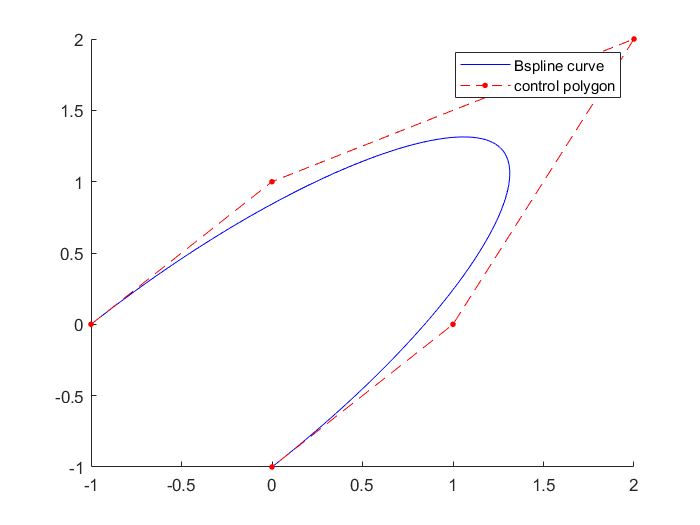
\includegraphics[width=0.8\textwidth]{bspline_2d_1.png}
        \label{fig: bspline_2d_1}
        \caption{控制顶点
        $p_0=(-1,0)', p_1=(0,1)', p_2=(2,2)', p_3=(1,0)', p_4=(0,-1)'$}
    \end{figure}
    \begin{figure}[H]
        \centering
        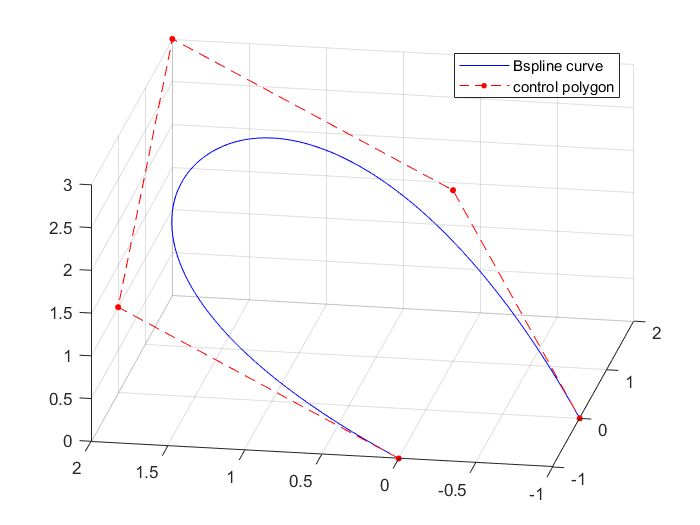
\includegraphics[width=0.8\textwidth]{bspline_3d_1.png}
        \label{fig: bspline_3d_1}
        \caption{控制顶点
        $p_0=(-1,0,0)', p_1=(0,2,1)', p_2=(2,2,3)', p_3=(1,0,2)', p_4=(0,-1,0)'$}
    \end{figure}
    \item 次数$p=2$,节点向量$u = [0, 0, 0, 1/3, 2/3, 1, 1, 1]$
    \begin{figure}[H]
        \centering
        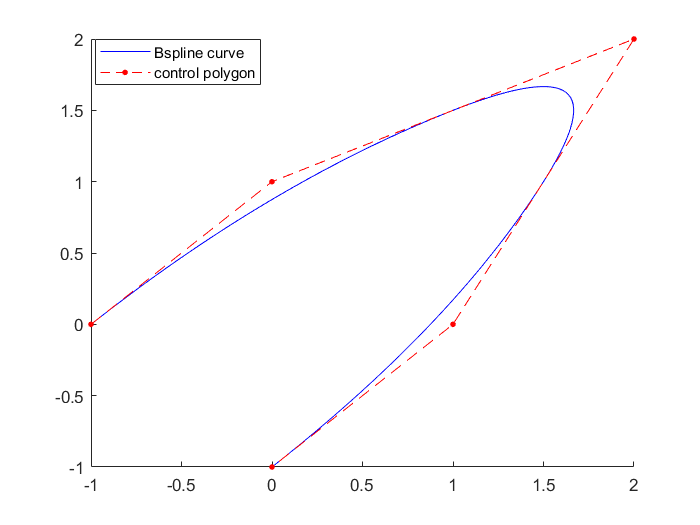
\includegraphics[width=0.8\textwidth]{bspline_2d_2.png}
        \label{fig: bspline_2d_2}
        \caption{控制顶点
        $p_0=(-1,0)', p_1=(0,1)', p_2=(2,2)', p_3=(1,0)', p_4=(0,-1)'$}
    \end{figure}
    \begin{figure}[H]
        \centering
        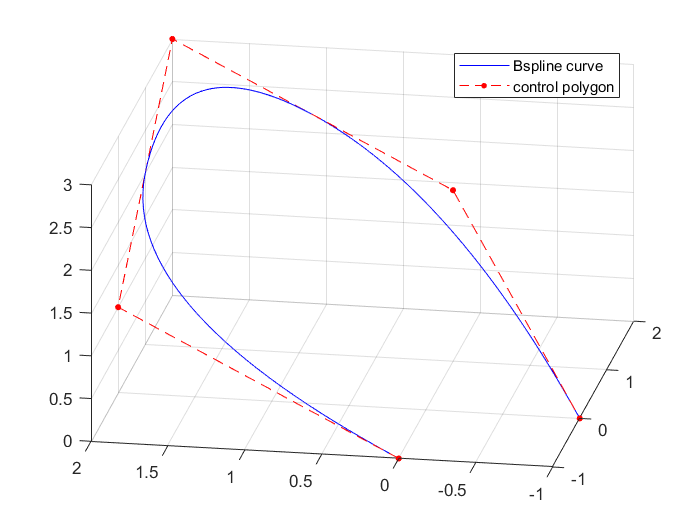
\includegraphics[width=0.8\textwidth]{bspline_3d_2.png}
        \label{fig: bspline_3d_2}
        \caption{控制顶点
        $p_0=(-1,0,0)', p_1=(0,2,1)', p_2=(2,2,3)', p_3=(1,0,2)', p_4=(0,-1,0)'$}
    \end{figure}
\end{itemize}


\end{document}
